\documentclass[USEnglish,ignorenonframetext,notheorems,aspectratio=1610]{beamer}
\usetheme[compress]{Madrid}
\usecolortheme{iwr}
\usepackage{tikz,tikzscale}
\usetikzlibrary{snakes}
\usepackage{../mathsim}
\usepackage{times}
\usepackage{xr}
\externaldocument{awa}
\externaldocument{explicit}
\externaldocument{implicit}
\externaldocument{lmm}
\externaldocument{rwa}
\externaldocument{newton}
\externaldocument{fd}
\externaldocument{appendix}
\usepackage{mfirstuc}
\usepackage{mathtools}  
\mathtoolsset{showonlyrefs}

\def\footnote#1{}

% Definitions for Runge-Kutta-Koefficients
\def\rks{s}  % Number of steps
\def\rka{a}  % Coefficient matrix
\def\rkb{b}  % Quadrature weights
\def\rkc{c}  % Quadrature points
\def\rkg{g}  % Intermediate points

\def\lmms{s}

% Definitions for boundary value problems
\def\rwaa{B_a}
\def\rwab{B_b}

\title{\textbf{Numerical Analysis \\of\\
    Ordinary Differential Equations}}
\author{Guido Kanschat}
\date{\today}
\begin{document}
\frame{\maketitle}
\frame{\frametitle{Overview}\tableofcontents[hideallsubsections]}
\section{Initial Value Problems and their Properties}
\frame{\tableofcontents[currentsection,hideothersubsections]}
\subsection{Modeling with ordinary differential equations}
\subsection{Introduction to initial value problems}

\frame {\input {blocks/Definition-ode.tex}}
\frame {\input {blocks/Definition-explicit-ode.tex}}
\frame {\input {blocks/Lemma-first-order.tex}}
\frame {\input {blocks/Definition-autonomization.tex}}
\frame {\input {blocks/Definition-IVP.tex}}
\frame {\input {blocks/Definition-local-solution.tex}}
\frame {\input {blocks/Lemma-volterra.tex}}
\frame {\input {blocks/Theorem-peano.tex}}
\frame {\input {blocks/Theorem-peano-continuation.tex}}

\subsection{Linear differential equations
  and Grönwall's inequality}

\frame {\input {blocks/Definition-linear-ode.tex}}
\frame {\input {blocks/Definition-integrating factor.tex}
  \input {blocks/Lemma-linear-representation.tex}}
\frame {\input {blocks/Lemma-gronwall.tex}}
\frame {\input {blocks/Corollary-awa:unique-linear.tex}}
\frame {\input {blocks/Lemma-solution-space.tex}}
\frame {\input {blocks/Definition-fundamental-system.tex}}
\frame {\input {blocks/Corollary-fundamental-regular.tex}}

\subsection{Well-posedness of the IVP}

\frame {\input {blocks/Definition-hadamard.tex}}
\frame {\input {blocks/Definition-Lipschitz-condition.tex}}
\frame {\input {blocks/Theorem-awa-stability.tex}}
\frame {\input {blocks/Theorem-picardlindelof.tex}}

\section{Explicit One-Step Methods and Convergence}
\frame{\tableofcontents[currentsection,hideothersubsections]}
\subsection{Introduction}

\frame {\input {blocks/Definition-partitioning.tex}}
\frame {\input {blocks/Definition-one-step.tex}}
\frame {\input {blocks/Example-euler-linear-1.tex}}

\subsection{Error analysis}
\begin{frame}
  \frametitle{Error decomposition}
  \centering
  \includegraphics[width=.49\textwidth]{fig/forward-error.tikz}
  \includegraphics[width=.49\textwidth]{fig/backward-error.tikz}
\end{frame}

\frame {\input {blocks/Definition-truncation-error.tex}}
\frame {\input {blocks/Lemma-gronwall-discrete.tex}}
\frame {\input {blocks/Theorem-stability-discrete.tex}}
\frame {\input {blocks/Corollary-finite-precision}}
\frame {\input {blocks/Theorem-convergence-one-step.tex}}

\subsection{Runge-Kutta methods}

\frame {\input {blocks/Definition-erk.tex}}
\frame {\input {blocks/Definition-butcher-tableau-erk.tex}}
\frame {\input {blocks/Example-rk2.tex}
  \input {blocks/Lemma-Heun-consistency.tex}}
\frame {\input {blocks/Example-rk3.tex}}
\frame {\input {blocks/Lemma-rk-order-3-4.tex}}
\frame {\input {blocks/Lemma-taylor-u.tex}}
\frame {\input {blocks/Lemma-taylor-y.tex}}
\frame {\input {blocks/Example-rk4.tex}}
\begin{frame}
  \begin{block}{Butcher barriers}
    \begin{tabular}{c|c|c|c|c|c|c|c|c|c|c|c}
  p & 1 & 2 & 3 & 4 & 5 & 6 & 7 & 8 & 9 & 10 \\\hline
  \# cond. & 1 & 2 & 4 & 8 & 17 & 37 & 85 & 200
  & 486 & 1205
  \\\hline
  \rks & p & p & p & p & p+1 & p+1 & p+2 & p+3 & ? & 17? \\
\end{tabular}    

%%% Local Variables: 
%%% mode: latex
%%% TeX-master: "../notes"
%%% End: 

  \end{block}
\end{frame}
\frame {\input {blocks/Lemma-erk-Lipschitz.tex}}

\subsection{Estimate of the truncation error and time step control}

\frame {\input {blocks/Theorem-richardson.tex}}
\frame {\input {blocks/Definition-embedded-butcher.tex}}
\frame {\input {blocks/Definition-dormand-prince-45.tex}}
\subsection{Continuous Runge-Kutta methods}

\frame {\input {blocks/Example-rk4-continuous.tex}}
\frame {\input {blocks/Example-dormand-prince-45-continuous.tex}}

\section{Implicit One-Step Methods and Long-Time Stability}
\frame{\tableofcontents[currentsection,hideothersubsections]}

\subsection{Monotonic initial value problem}

\frame {\input {blocks/Definition-lipschitz-one-sided.tex}}
\frame {\input {blocks/Theorem-stability-monotonic.tex}}
\frame {\input {blocks/Lemma-linear-monotonic.tex}}
\frame {\input {blocks/Definition-stiff.tex}}

\subsection{A- and B-stability}

\frame {\input {blocks/Definition-stability-function.tex}}

\begin{frame}
  \frametitle{Stability regions of the implicit and explicit Euler
    methods}
  \begin{center}
    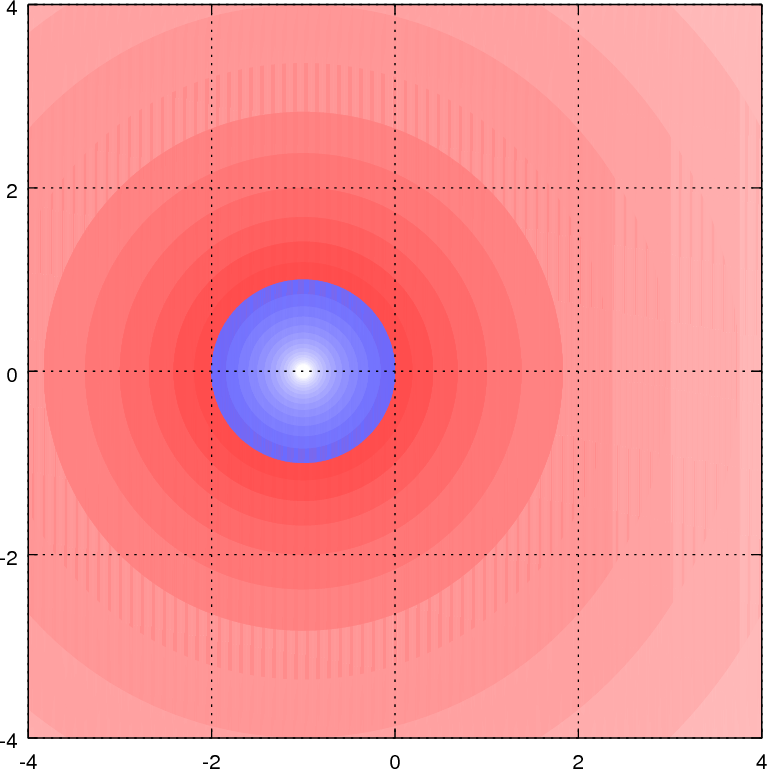
\includegraphics[width=.47\textwidth]{fig/stability-euler}
    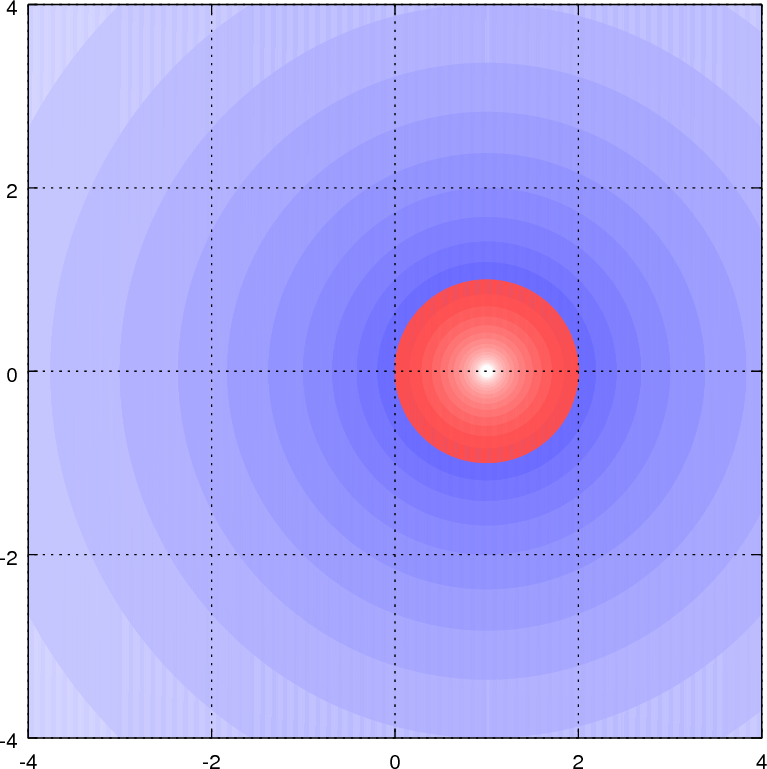
\includegraphics[width=.47\textwidth]{fig/stability-euler2}
  \end{center}
\end{frame}

\frame {\input {blocks/Definition-a-stability.tex}
  \input {blocks/Theorem-a-stability.tex}}
\frame {\input {blocks/Theorem-implicit:a-stability-erk.tex}}
\frame {\input {blocks/Definition-b-stability.tex}}
\frame {\input {blocks/Theorem-b-stability.tex}
  \input {blocks/Corollary-b-stable-a-stable.tex}}
\frame {\input {blocks/Definition-l-stability.tex}}

\subsection{General Runge-Kutta methods}

\frame {\input {blocks/Definition-rk.tex}}
\begin{frame}
  \begin{block}{Two-stage SDIRK methods of order 3}
    \begin{gather*}
      \def\arraystretch{1.5}
      \begin{array}{c|cc}
        \frac12 - \frac{\sqrt{3}}{6} & \frac12 - \frac{\sqrt{3}}{6} & 0 \\
        \frac12 + \frac{\sqrt{3}}{6} & \frac{\sqrt{3}}{3} & \frac12 - \frac{\sqrt{3}}{6} \\
        \hline
                                     & \frac12 & \frac12
      \end{array}
      \qquad
      \begin{array}{c|cc}
        \frac12 + \frac{\sqrt{3}}{6} & \frac12 + \frac{\sqrt{3}}{6} & 0 \\
        \frac12 - \frac{\sqrt{3}}{6} & -\frac{\sqrt{3}}{3} & \frac12 + \frac{\sqrt{3}}{6} \\
        \hline
                                     & \frac12 & \frac12
      \end{array}
    \end{gather*}
  \end{block}  
\end{frame}
\frame {\input {blocks/Lemma-stability-rk.tex}}
\frame {\input {blocks/Example-stability-examples-rk.tex}}

\begin{frame}
  \frametitle{Stability domains of ERK}
  \begin{tabular}{ccc}
    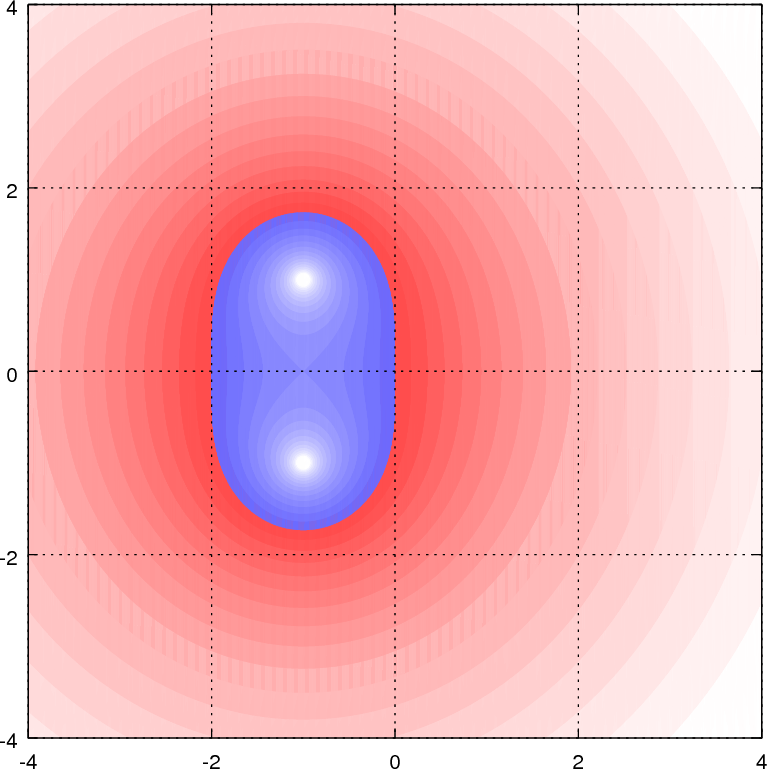
\includegraphics[width=.3\textwidth]{fig/stability-RK2}
    &
    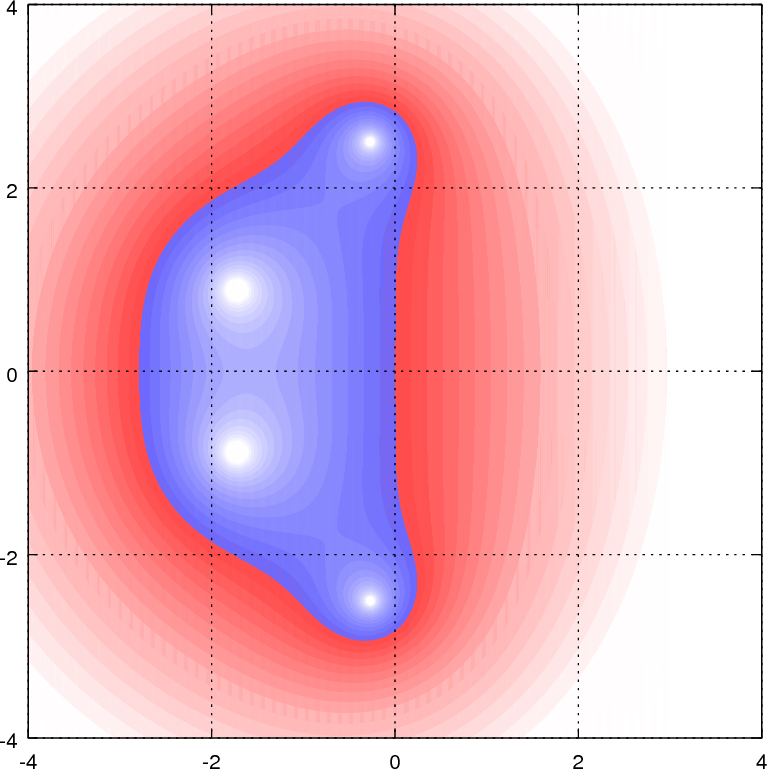
\includegraphics[width=.3\textwidth]{fig/stability-RK4}
    &
    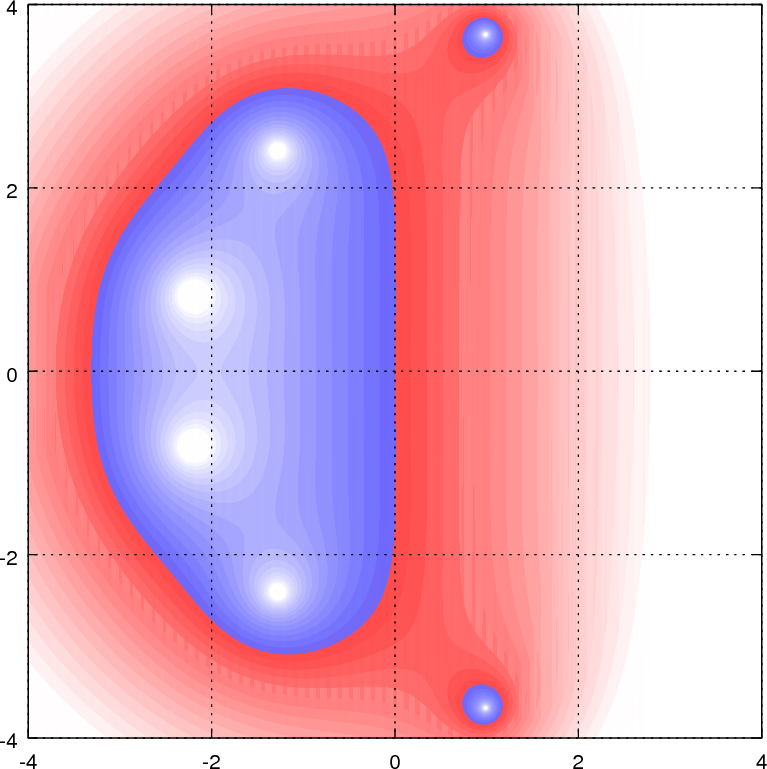
\includegraphics[width=.3\textwidth]{fig/stability-DOPRI5}
    \\
    mod. Euler & RK4 & DOPRI5
  \end{tabular}
\end{frame}

\frame {\input {blocks/Definition-theta-scheme.tex}}
\frame {\input {blocks/Theorem-theta-a-stability.tex}}

\begin{frame}
  \frametitle{Stability domains of the $\theta$-scheme}
  \begin{center}
    \begin{tabular}{cccc}
      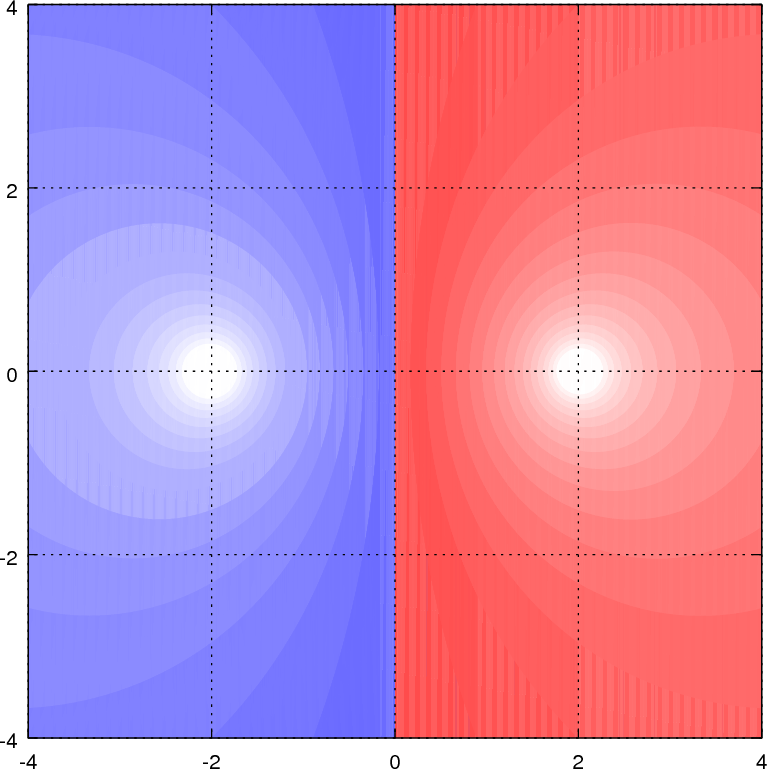
\includegraphics[width=.22\textwidth]{fig/stability-CR}
      &
      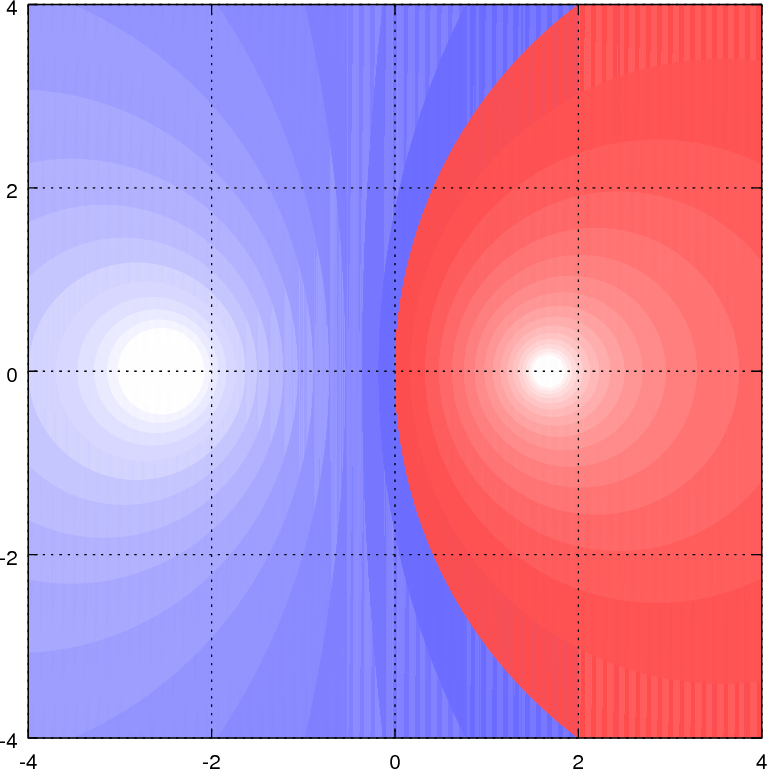
\includegraphics[width=.22\textwidth]{fig/stability-theta6}
      &
      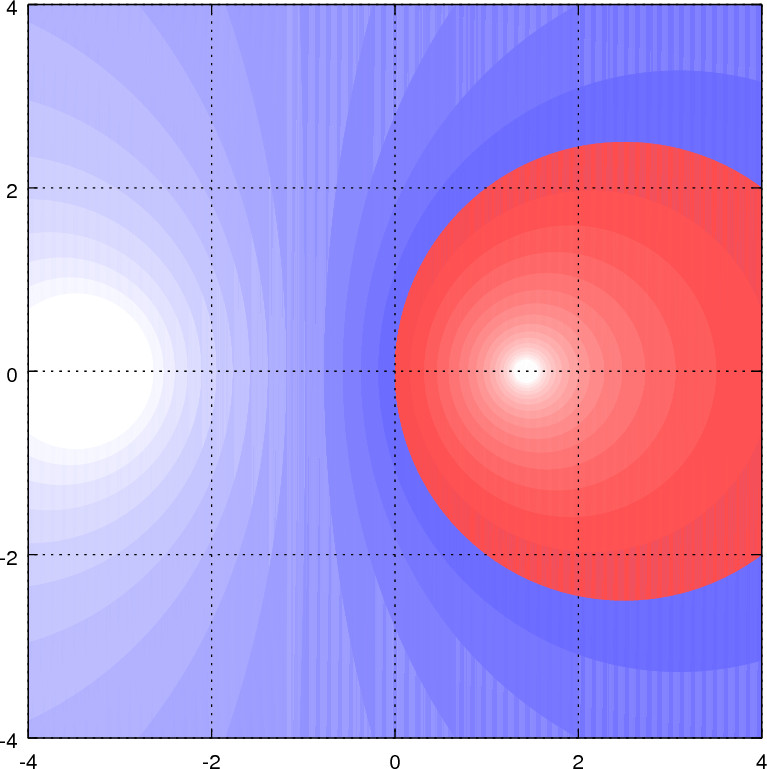
\includegraphics[width=.22\textwidth]{fig/stability-theta7}
      &
      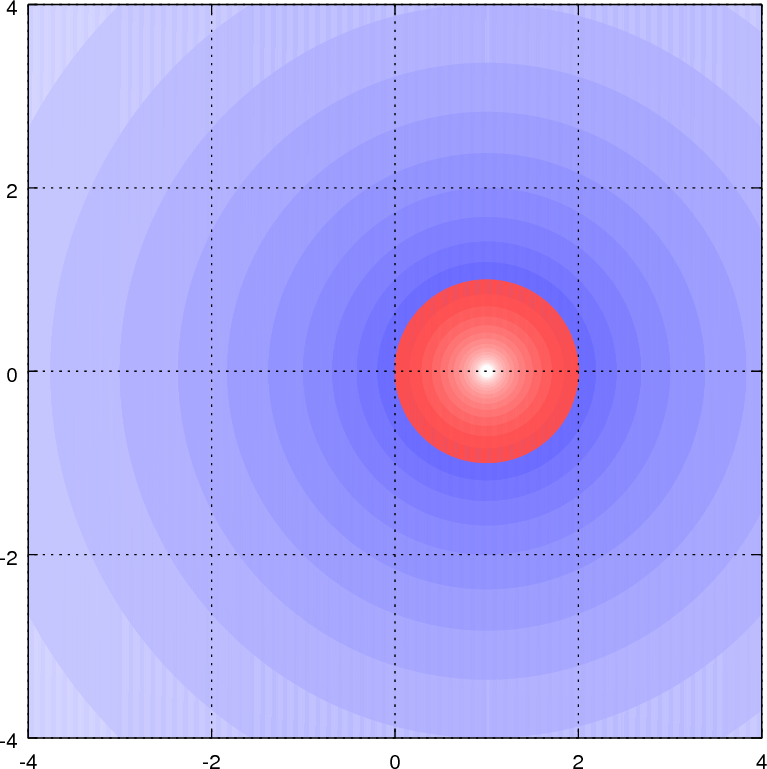
\includegraphics[width=.22\textwidth]{fig/stability-euler2}
      \\
      $\theta= 0.5$
      & $\theta = 0.6$
      & $\theta = 0.7$
      & $\theta = 1.0$
      \\
      Crank-Nicolson &&& impl. Euler
    \end{tabular}
  \end{center}
\end{frame}

\frame {\input {blocks/Lemma-existence-implicit-1.tex}}
\frame {\input {blocks/Lemma-existence-implicit-2.tex}}
\frame {\input {blocks/Theorem-existence-implicit-3.tex}}
\frame {\input {blocks/Definition-simplifying-conditions.tex}
  \input {blocks/Theorem-order-conditions.tex}}

\subsection{Methods based on quadrature}

\frame {\input {blocks/Definition-gauss-quadrature.tex}}
\frame {\input {blocks/Definition-radau-lobatto-quadrature.tex}}
\frame {\input {blocks/Lemma-gauss-quadrature.tex}}
\frame {\input {blocks/Definition-collocation.tex}}
\frame {\input {blocks/Lemma-collocation.tex}}
\frame {\input {blocks/Lemma-collocation-equivalence.tex}}
\frame {\input {blocks/Theorem-collocation-order.tex}}
\frame {\input {blocks/Theorem-collocation-continuous.tex}}
\frame {\input {blocks/Definition-gauss-collocation.tex}}
\frame {\input {blocks/Example-Gauss-collocation-2-3.tex}}
\frame {\input {blocks/Theorem-gauss-consistency.tex}
  \input {blocks/Theorem-gauss-stability.tex}}
\frame {\input {blocks/Example-Radau-right-2-3.tex}}
\begin{frame}
  \frametitle{Stability regions of Radau-collocation methods}
    \centering
  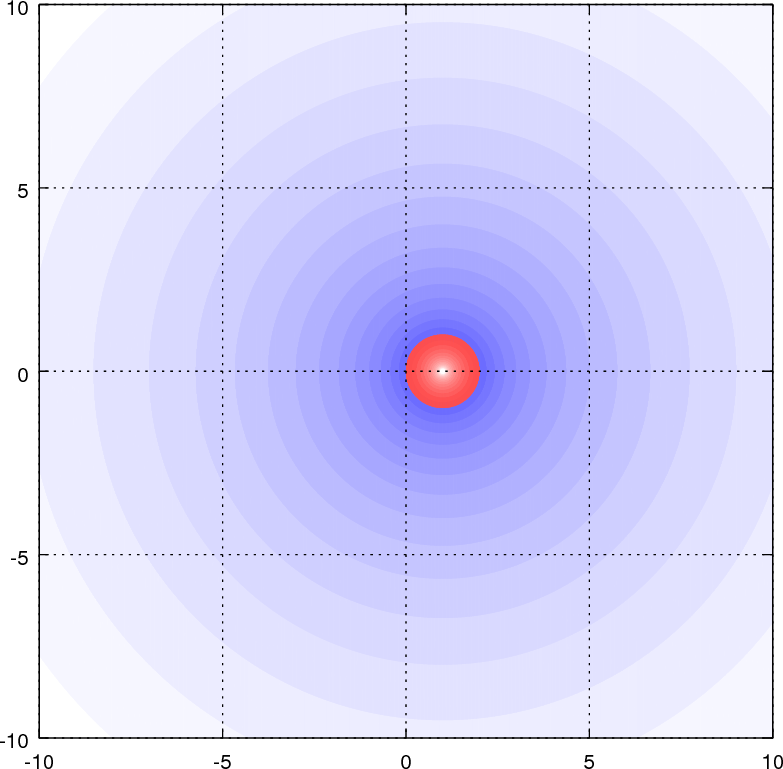
\includegraphics[width=.3\textwidth]{fig/stability-radau1}
  \hfill
  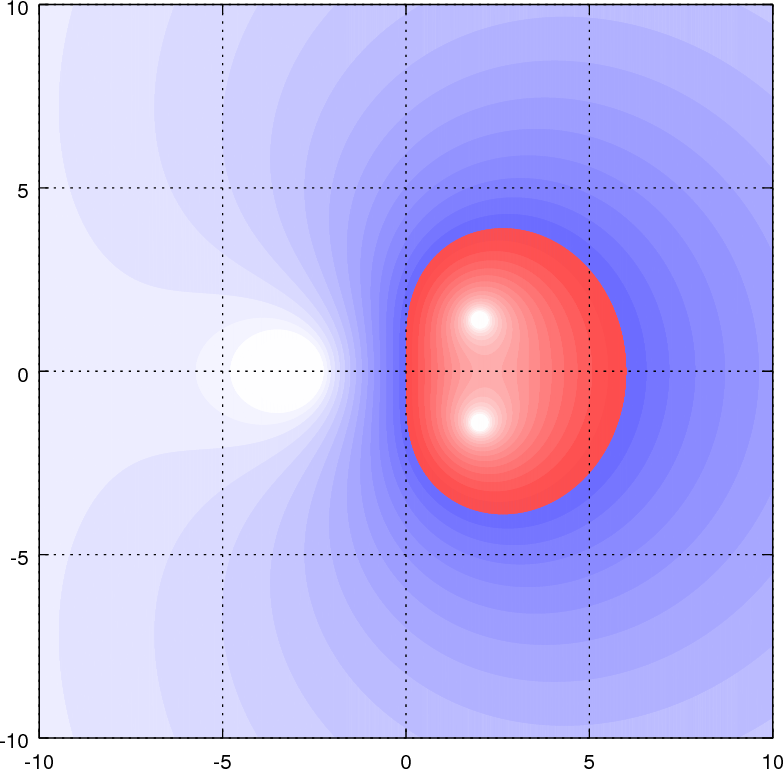
\includegraphics[width=.3\textwidth]{fig/stability-radau2}
  \hfill
  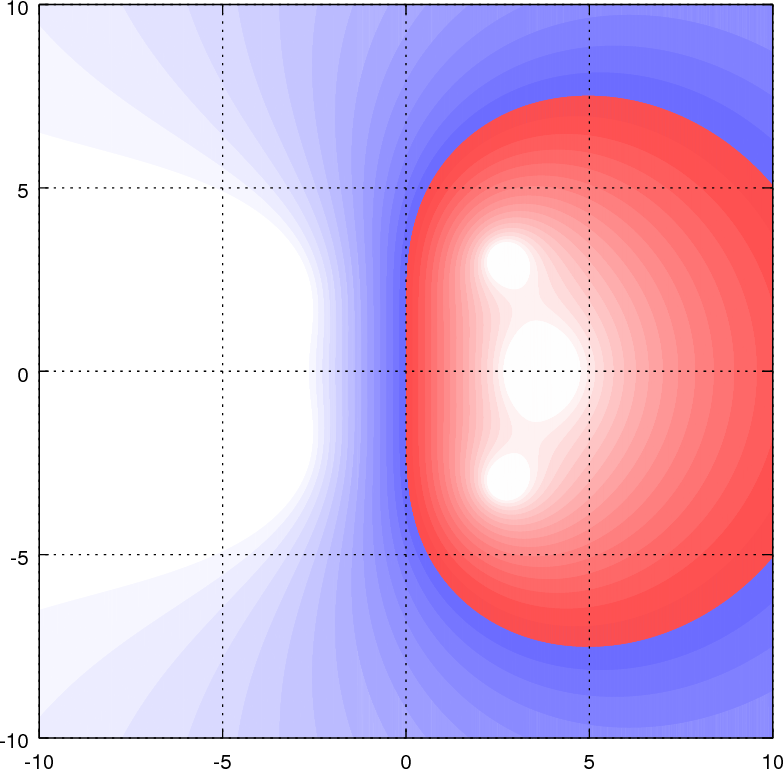
\includegraphics[width=.3\textwidth]{fig/stability-radau3}
\end{frame}

\frame {\input {blocks/Theorem-DIRK-order-barrier.tex}}

\section{Newton and quasi-Newton methods}

\frame {\input {blocks/Definition-nonlinear.tex}}
\frame {\input {blocks/Definition-iteration-order.tex}}
\frame {\input {blocks/Definition-newton.tex}}
\frame {\input {blocks/Theorem-newton-kantorovich.tex}}
\frame {\input {blocks/Definition-gradient-method.tex}}
\frame {\input {blocks/Theorem-gradient-method.tex}}
\frame {\input {blocks/Definition-newton-line-search.tex}}
\frame {\input {blocks/Definition-newton-step-size.tex}}
\frame {\input {blocks/Definition-descent-methods.tex}}
\frame {\input {blocks/Lemma-downhill.tex}}


\section{Linear Multi-Step Methods}
\frame{\tableofcontents[currentsection,hideothersubsections]}

\begin{frame}
  \begin{block}{Adams-Moulton methods (implicit)}
  \begin{gather*}
    y_k = y_{k-1} + \sum_{r=0}^\lmms f_{k-r} \int_{t_{k-1}}^{t_k}
    L_r(t) \dt,
  \end{gather*}
    \begin{center}
      \includegraphics[width=.9\textwidth]{fig/adams-moulton.tikz}
    \end{center}
    \begin{align*}
  y_k &= y_{k-1} + h f_k \\
  y_k &= y_{k-1} + \frac12h
        \bigl( f_k + f_{k-1}\bigr)\\
  y_k &= y_{k-1} +
        \frac1{12}h \bigl( 5f_k + 8 f_{k-1} -  f_{k-2}\bigr)\\
  y_k &= y_{k-1} +
        \frac1{24}h \bigl(9f_k+19 f_{k-1}-5 f_{k-2}+ f_{k-3}\bigr)
\end{align*}

%%% Local Variables:
%%% mode: latex
%%% TeX-master: "../notes"
%%% End:
    
  \end{block}
\end{frame}
\begin{frame}
  \begin{block}{Adams-Bashforth methods (explicit)}
  \begin{gather*}
    y_k = y_{k-1} + \sum_{r=1}^\lmms f_{k-r} \int_{t_{k-1}}^{t_k}
    L_r(t) \dt.
  \end{gather*}
    \begin{center}
      \includegraphics[width=.9\textwidth]{fig/adams-bashforth.tikz}
    \end{center}
    \begin{tikzpicture}
  \draw[snake=snake](7,0) -- (8,0);
  \draw(5,0) -- (7,0);
  % \draw(2,0) -- (3,0);
  \draw[dotted](0,0)--(3,0);
  \draw[dashed](3,0)--(5,0);
  
  \draw(8,-.1) --(8,.1) node[anchor=south]{$t_{k}$};
  \draw(7,-.1) node[anchor=north]{$t_{k-1}$} --(7,.1);
  \draw(6,-.1) node[anchor=north]{$t_{k-2}$} --(6,.1);
  \draw(5,-.1) node[anchor=north]{$t_{k-3}$} --(5,.1);
  
  \draw(3,-.1) node[anchor=north]{$t_{k-\lmms}$} --(3,.1);
  % \draw(2,-.1) --(2,.1) node[anchor=south]{$t_{k-\lmms-1}$};
\end{tikzpicture}

  \end{block}
\end{frame}
\begin{frame}
  \begin{block}{Backward Differencing Formulas}
  \begin{gather*}
    y'(t_k) = f(t_k, y_k) = \sum_{r=0}^\lmms y_{k-r} L'_{k-r}(t_k).
  \end{gather*}
    \begin{align*}
  y_k-y_{k-1} &= h f_k \\
  y_k-\tfrac43 y_{k-1} + \tfrac13y_{k-2} &= \tfrac23 h f_k \\
  y_k-\tfrac{18}{11} y_{k-1} + \tfrac{9}{11} y_{k-2} -
  \tfrac{2}{11} y_{k-3}
              &= \tfrac6{11} h f_k \\
  y_k-\tfrac{48}{25} y_{k-1} + \tfrac{36}{25} y_{k-2} -
  \tfrac{16}{25} y_{k-3} + \tfrac{3}{25} y_{k-4}
              &= \tfrac{12}{25} h f_k
\end{align*}

%%% Local Variables:
%%% mode: latex
%%% TeX-master: "../notes"
%%% End:

  \end{block}
\end{frame}

\frame {\input {blocks/Definition-lmm.tex}}
\frame {\input {blocks/Definition-lmm-errors.tex}}
\frame {\input {blocks/Definition-lmm-consistency.tex}}
\frame {\input {blocks/Lemma-lmm-bramble-hilbert.tex}}
\frame {\input {blocks/Theorem-lmm-consistency.tex}}
\frame {\input {blocks/Definition-difference-equation.tex}}
\frame {\input {blocks/Lemma-lmm:1.tex}}
\frame {\input {blocks/Lemma-difference-equation-solutions.tex}}
\frame {\input {blocks/Theorem-difference-equation-basis.tex}}
\frame {\input {blocks/Corollary-root-test.tex}}
\frame {\input {blocks/Definition-lmm-stability.tex}
  \input {blocks/Theorem-lmm-stability.tex}}
\frame {\input {blocks/Corollary-adams-stability}
  \input {blocks/Theorem-BDF-stability.tex}}
\frame {\input {blocks/Definition-lmm-convergence.tex}}
\frame {\input {blocks/Lemma-lmm-one-step.tex}}
\frame {\input {blocks/Lemma-lmm-one-consistency.tex}}
\frame {\input {blocks/Lemma-lmm-one-stability.tex}}
\frame {\input {blocks/Theorem-lmm-convergence.tex}}
\frame {\input {blocks/Definition-lmm-stability-region.tex}}
\frame {\input {blocks/Definition-lmm-stability-polynomial.tex}
  \input {blocks/Lemma-lmm-stability.tex}}
\frame {\input {blocks/Theorem-dahlquist2.tex}}
\frame {\input {blocks/Definition-aa-stability.tex}}

\frame{
\begin{figure}[tp]
  \centering
  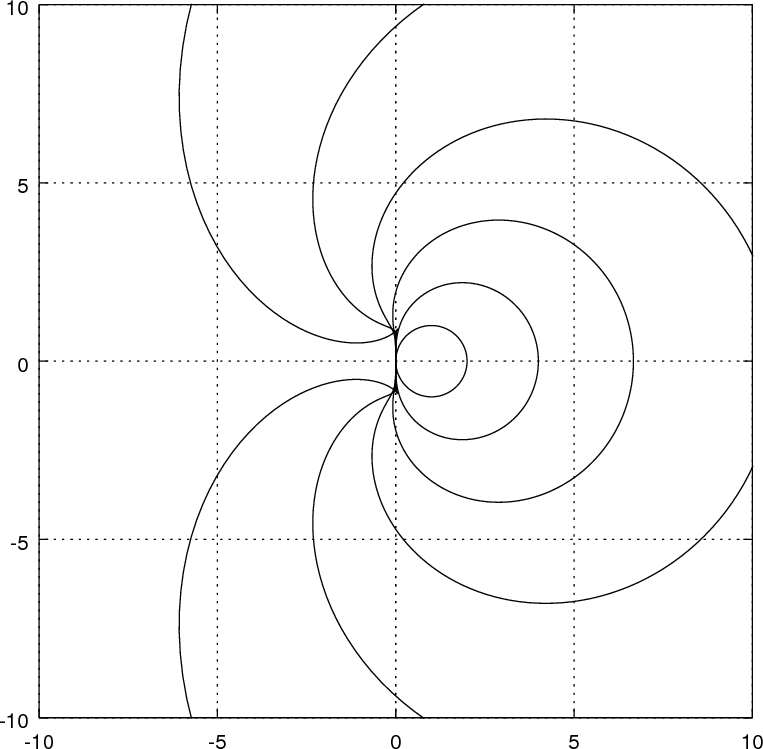
\includegraphics[width=.45\textwidth]{fig/stability-bdf.png}
  \hfill
  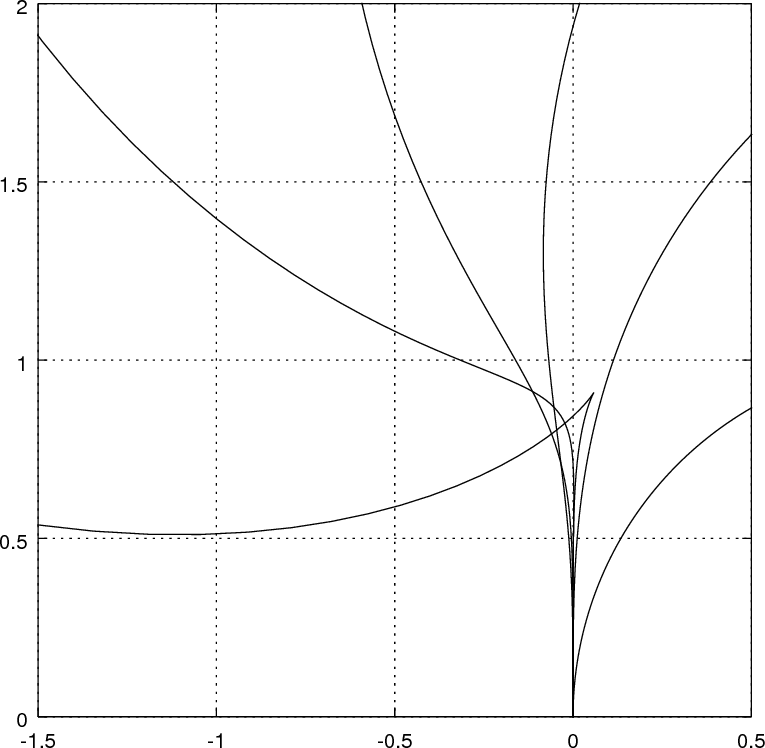
\includegraphics[width=.45\textwidth]{fig/stability-bdf-zoom.png}
  \caption{Boundaries of stability regions of BDF1 to BDF6. Unstable
    region right of the origin. Zoom on the right}
  \label{fig:bdf-stability}
\end{figure}
}

\frame {\input {blocks/Definition-predictor-corrector.tex}}

\section{Boundary Value Problems}
\frame{\tableofcontents[currentsection,hideothersubsections]}

\frame {\input {blocks/Definition-bvp.tex}}
\frame {\input {blocks/Definition-bvp-linear.tex}}
\frame {\input {blocks/Definition-gateaux-derivative.tex}}
\frame {\input {blocks/Definition-variational-equation.tex}}
\frame {\input {blocks/Lemma-fundamental.tex}}
\frame {\input {blocks/Theorem-derivative.tex}}
\frame {\input {blocks/Theorem-derivative-f.tex}}
\frame {\input {blocks/Definition-local-uniqueness.tex}}
\frame {\input {blocks/Lemma-bvp-derivative.tex}}
\frame {\input {blocks/Theorem-local-uniqueness.tex}}
\frame {\input {blocks/Theorem-bvp-stability-1.tex}}
\frame {\input {blocks/Theorem-bvp-stability-2.tex}}
\frame {\input {blocks/Corollary-bvp-linear.tex}}
\frame {\input {blocks/Definition-single-shooting.tex}}
\frame {\input {blocks/Algorithm-single-shooting.tex}}
\frame {\input {blocks/Definition-multiple-shooting.tex}}
\frame {\input {blocks/Definition-multiple-shooting-newton.tex}}
\frame {\input {blocks/Definition-multiple-shooting-multiple.tex}}
\frame {\input {blocks/Definition-bvp-parameter.tex}}
\frame {\input {blocks/Definition-multiple-shooting-parameter.tex}}

\section{Finite Differences}
\frame{\tableofcontents[currentsection,hideothersubsections]}

\frame {\input {blocks/Definition-bvp-second.tex}}
\frame {\input {blocks/Definition-difference-operators.tex}}
\frame {\input {blocks/Definition-fd-consistency.tex}}
\frame {\input {blocks/Lemma-fd-consistency.tex}}
\frame {\input {blocks/Definition-fd.tex}}
\frame {\input {blocks/Example-fd-example.tex}}
\frame {\input {blocks/Example-fd-matrix.tex}}

\begin{frame}
  \begin{block}{The reduced system}
    \begin{gather*}
      L_h y =
    \begin{pmatrix}
      \lambda_1 & \nu_1\\
      \mu_2 & \lambda_2 & \nu_2 \\
      & \ddots & \ddots & \ddots \\
      &&\mu_{n-1}& \lambda_{n-1}
    \end{pmatrix}
    \begin{pmatrix}
      y_1\\\vdots\\y_{n-1}
    \end{pmatrix}
    =
    \begin{pmatrix}
      f_1 \\\vdots\\f_{n-1}
    \end{pmatrix} = f_h.
  \end{gather*}
  \end{block}
\end{frame}

\frame {\input {blocks/Definition-m-matrix.tex}}
\frame {\input {blocks/Lemma-m-matrix-fd1.tex}}
\frame {\input {blocks/Lemma-m-matrix-inverse.tex}}
\frame {\input {blocks/Theorem-fd-stability.tex}}
\frame {\input {blocks/Example-upwind.tex}}
\frame {\input {blocks/Theorem-fd-convergence.tex}}
\frame {\input {blocks/Example-square-domain.tex}}
\frame {\input {blocks/Definition-laplace-equation.tex}}
\frame {\input {blocks/Example-dirichlet.tex}}
\frame {\input {blocks/Theorem-mean-value.tex}}
\frame {\input {blocks/Theorem-maximum.tex}}
\frame {\input {blocks/Definition-cartesian-grid.tex}}
\frame {\input {blocks/Definition-lexicographic.tex}}
\frame {\input {blocks/Definition-5-point-stencil.tex}}
\frame {\input {blocks/Lemma-fd-matrix.tex}}
\frame {\input {blocks/Theorem-5-point-m-matrix.tex}}
\frame {\input {blocks/Lemma-fd2-consistency.tex}}
\frame {\input {blocks/Theorem-fd2-convergence.tex}}
\frame {\input {blocks/Theorem-fd2-maximum.tex}}

\end{document}

%%% Local Variables:
%%% mode: latex
%%% TeX-master: t
%%% End:
